TODO intro


\subsection{CPUID Instruction}
\label{sec:approach-cpuid}

\mvf{Draft:}

P{\'e}k {\em et al.}~\cite{nether}

Ether alters the output of {\tt CPUID}, flipping the bit for TSC support. Should
be 1 in both VMM and bare metal environment. Can easily be checked, as shown in
Figure~\ref{fig:cpuid-tsc}, in the Appendix.

If it is a bug in the Ether implementation, best solution is to fix, though we
do not have good enough knowledge of the source code to know.

Alternatively, spoof the value in the same manner as {\tt PUSHF} and {\tt POPF}.
Ether deliberately changes the flag register when running, as it sets the debug
flag to be able to step through the target program and get a program trace. It
hides this from the target by spoofing the values of instructions used to read
and write these flags, as {\tt PUSHF} and {\tt POPF}. Figure~\ref{fig:pushf}
shows how the Xen hypervisor is patched to check for specific instructions and
alter the effect of that instruction. The exact same technique could be used to
spoof the TSC-bit when program executes CPUID.

This technique of spoofing the CPUID output suffers from timing attacks, which
will be elaborated in~\nameref{sec:approach-timing}.

\begin{figure}
\begin{lstc}
void vmx_set_pending_exceptions(struct vcpu *v)
{
    ...
+    if(instruction[0] == 0x9C)
+    {
+         /* detected PUSHF */
+
+         v->domain->arch.hvm_domain.ether_controls.send_guest_exception = 1;
+         v->domain->arch.hvm_domain.ether_controls.next_expected_rip = guest_rip + 1;
+    }
+    else if (instruction[0] == 0x9D)
+    {
+         /* detected POPF */
+         ...
+    }
    ...
}
\end{lstc}
\caption{\label{fig:pushf} Part of the patch Ether does on the }
\end{figure}

\subsection{CPU Errata}
\label{sec:approach-errata}
CPU errata refer to the collection of design defects or errors that may induce the CPU to behave differently from the published specification. Such CPU errata is strongly bound to CPU models and nEther exploits bugs in the Core 2 Duo family, called AH4 Erratum. The AH4 Erratum states that "VERW/VERR/LSL/LAR" instructions may unexpectedly update the Last Exception Record(LER) MSR" and there is no planned fix for it. Concretely, VERW and VERR instructions verify whether the code or data segment specified with the source operand is readable (VERR) or writable (VERW) from the current privilege level. The LAR instruction loads access rights from a segment descriptor into a general purpose register, and the LSL instruction loads the unscrambled segment limit from the segment descriptor into a general-purpose register~\cite{intelsys}. This erratum is a design fault so its existence is unintended. Therefore, hardware-assisted-virtualization solutions (e.g., Xen) will not implement this erratum in the virtual CPUs of guests, because there is no need to mimic even unexpected system bugs. As a result, malware can detect hardware-assisted virtualization environment by executing those buggy instructions and checking whether LER MSR is unexpectedly updated or not. In other words, this attack cannot recognize the presence of Ether, but can reveal the hardware-virtualized runtime environment. \\

To thwart this attack completely, we should patch those buggy instructions or use another CPU, but It seems like infeasible and make no sense. So, we propose two practical method to mitigate this attack.

\begin{figure}[!h]
	\centering
	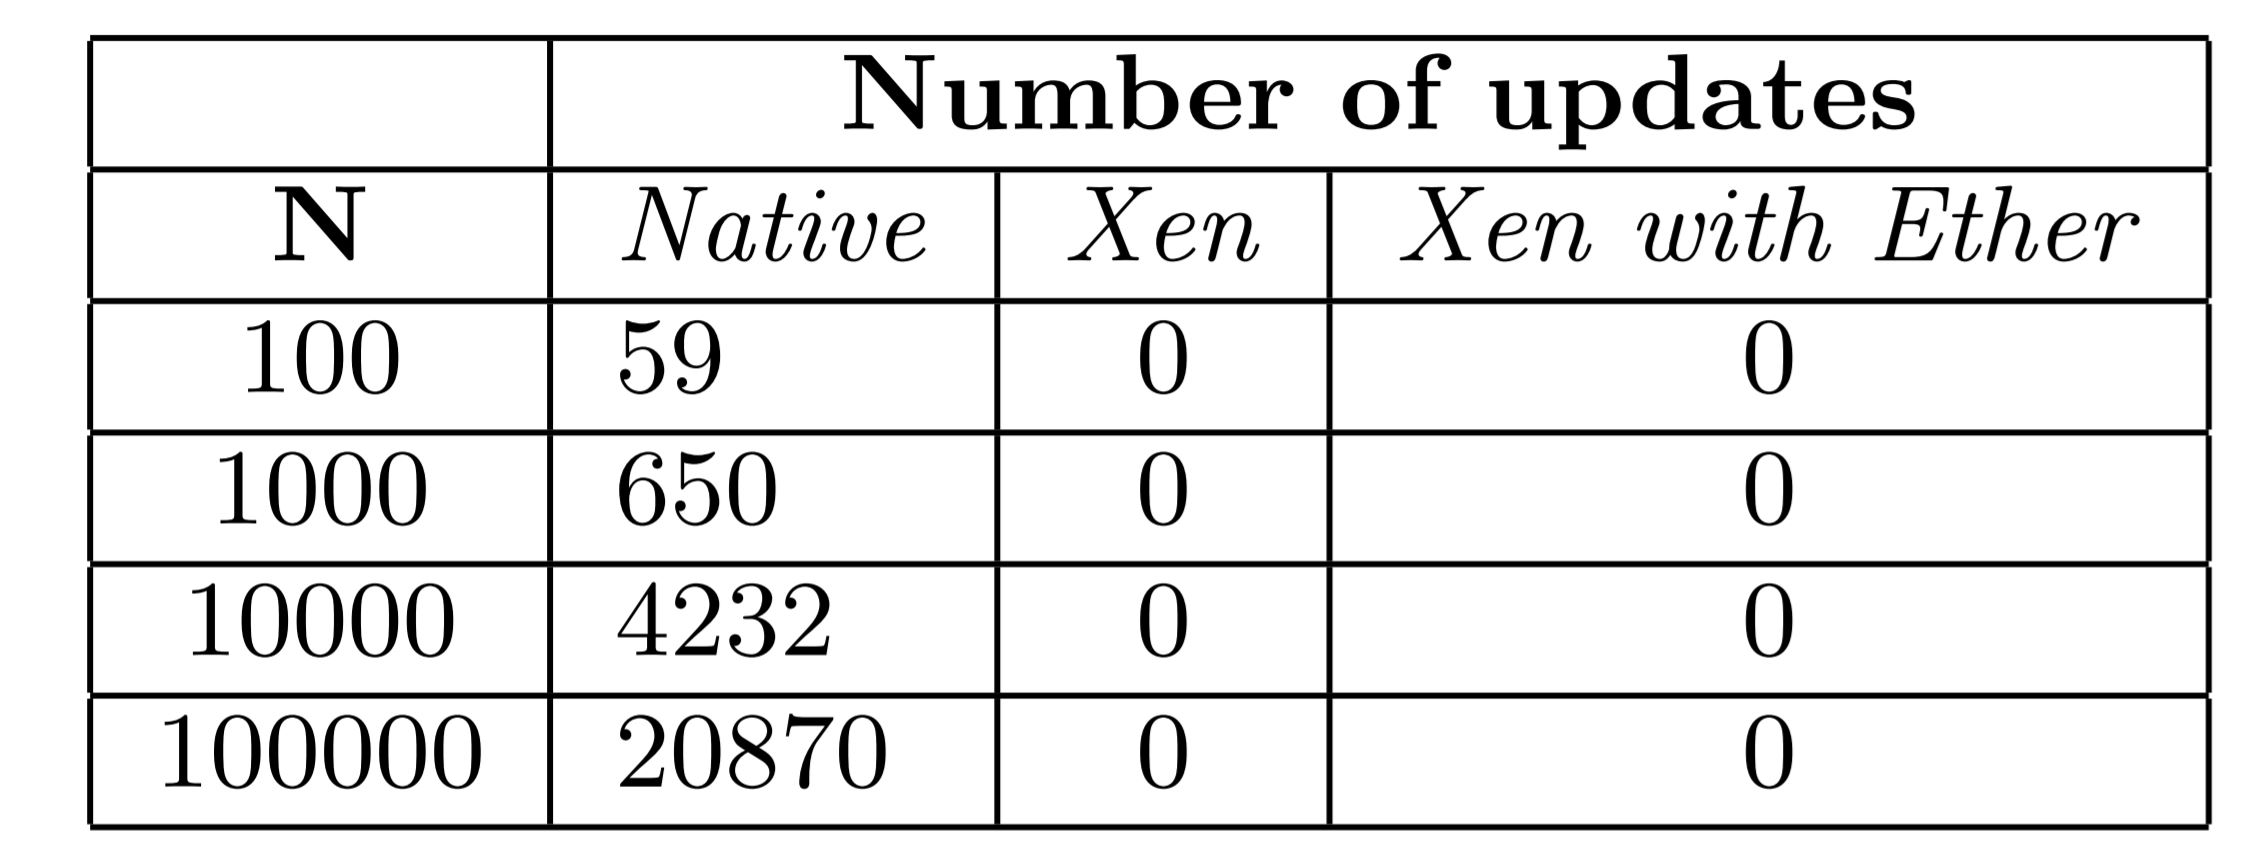
\includegraphics[width=\linewidth]{figure/errata_table.png}
	\caption{The number of LER MSR updates according to the erratum execution}
	\label{fig:errata}
\end{figure}

\subsubsection{Proposed Mitigation 1}
In general, those bugs do not happen always. Table~\ref{fig:errata} demonstrates the number of LER MSR updates when the CPU erratum was executed 100, 1000, 10000 and 100000 times under the corresponding environments. The update occurs only in the native environment, but the frequency of occurrence is unpredictable and irregular(from 20\% up to 65\%). Therefore, this CPU erratum should be executed in several times in order to detect hardware-assisted virtualization environment and this can be considered as a malicious behavior. So, to mitigate this attack, we set the threshold first and then count the number of all execution about those buggy instructions during the runtime of each program. If the counted number exceed the threshold, we can classify that program as a malware or just block to execute buggy instructions anymore. This method cannot prevent from CPU errata attack but can mitigate it, and there is a trade-off between TP and FP depending on how the threshold is set. Note that only kernel mode operations can access to LER MSR, therefore user mode operations does not need to be blocked or classified as a malware, even if execute the CPU erratum unlimited.

\subsubsection{Proposed Mitigation 2}
Another proposed mitigation is to mimic the CPU erratum intentionally. 

\subsection{Timing Information}
\label{sec:approach-timing}
Taking advantage to the performance and timing information is more sophisticated method for malwares to detect its environment. Although virtual machine\textquotesingle s performance is always slower than it would have been on real hardware, blindly measuring the absolute performance scores is not enough to determine whether its environment. Generally, two approaches to use timing information.



%%% Local Variables:
%%% mode: latex
%%% TeX-master: "../paper"
%%% End:
